\documentclass[12pt]{article}
\usepackage[letterpaper, margin=1in]{geometry}
\usepackage{graphicx}
\graphicspath{{./Figures/}}
\usepackage{hyperref}
\usepackage{parskip}
\usepackage{amsmath}
\usepackage{caption}
\usepackage{subcaption}
\usepackage[framed, numbered]{matlab-prettifier}
\lstset{inputpath=../MATLAB}

\DeclareMathOperator{\sinc}{sinc}
\DeclareMathOperator{\rect}{rect}

\title{ELECENG 3TR4 Lab 4: \\ Random Processes}
\author{
    Aaron Pinto \\ pintoa9
    \and
    Raeed Hassan \\ hassam41
}

% \lstinputlisting[style=Matlab-editor, caption={}, label={}, linerange={}]{Lab4.m} % for reference

\begin{document}

\maketitle
\clearpage

\section*{Numerical Experiment \#1: Evaluation of Autocorrelation and Power Spectral Density}

% (i) calculate the theoretical autocorrelation function of the output, and the corresponding PSD using the methodology discussed in class. Compare (qualitatively) your theoretical results with those from your program, and explain any discrepancies. Note that the amplitude (i.e. y-axis) of PSD of the matlab could be different from that of the theoretical PSD because of the difference between DFT and Fourier transform.

% (ii) change the maxlag from 100 to 200 and then to 500 and observe its impact on the PSD and comment. Include plots of all relevant quantities.

\begin{figure}[h]
	\centering
	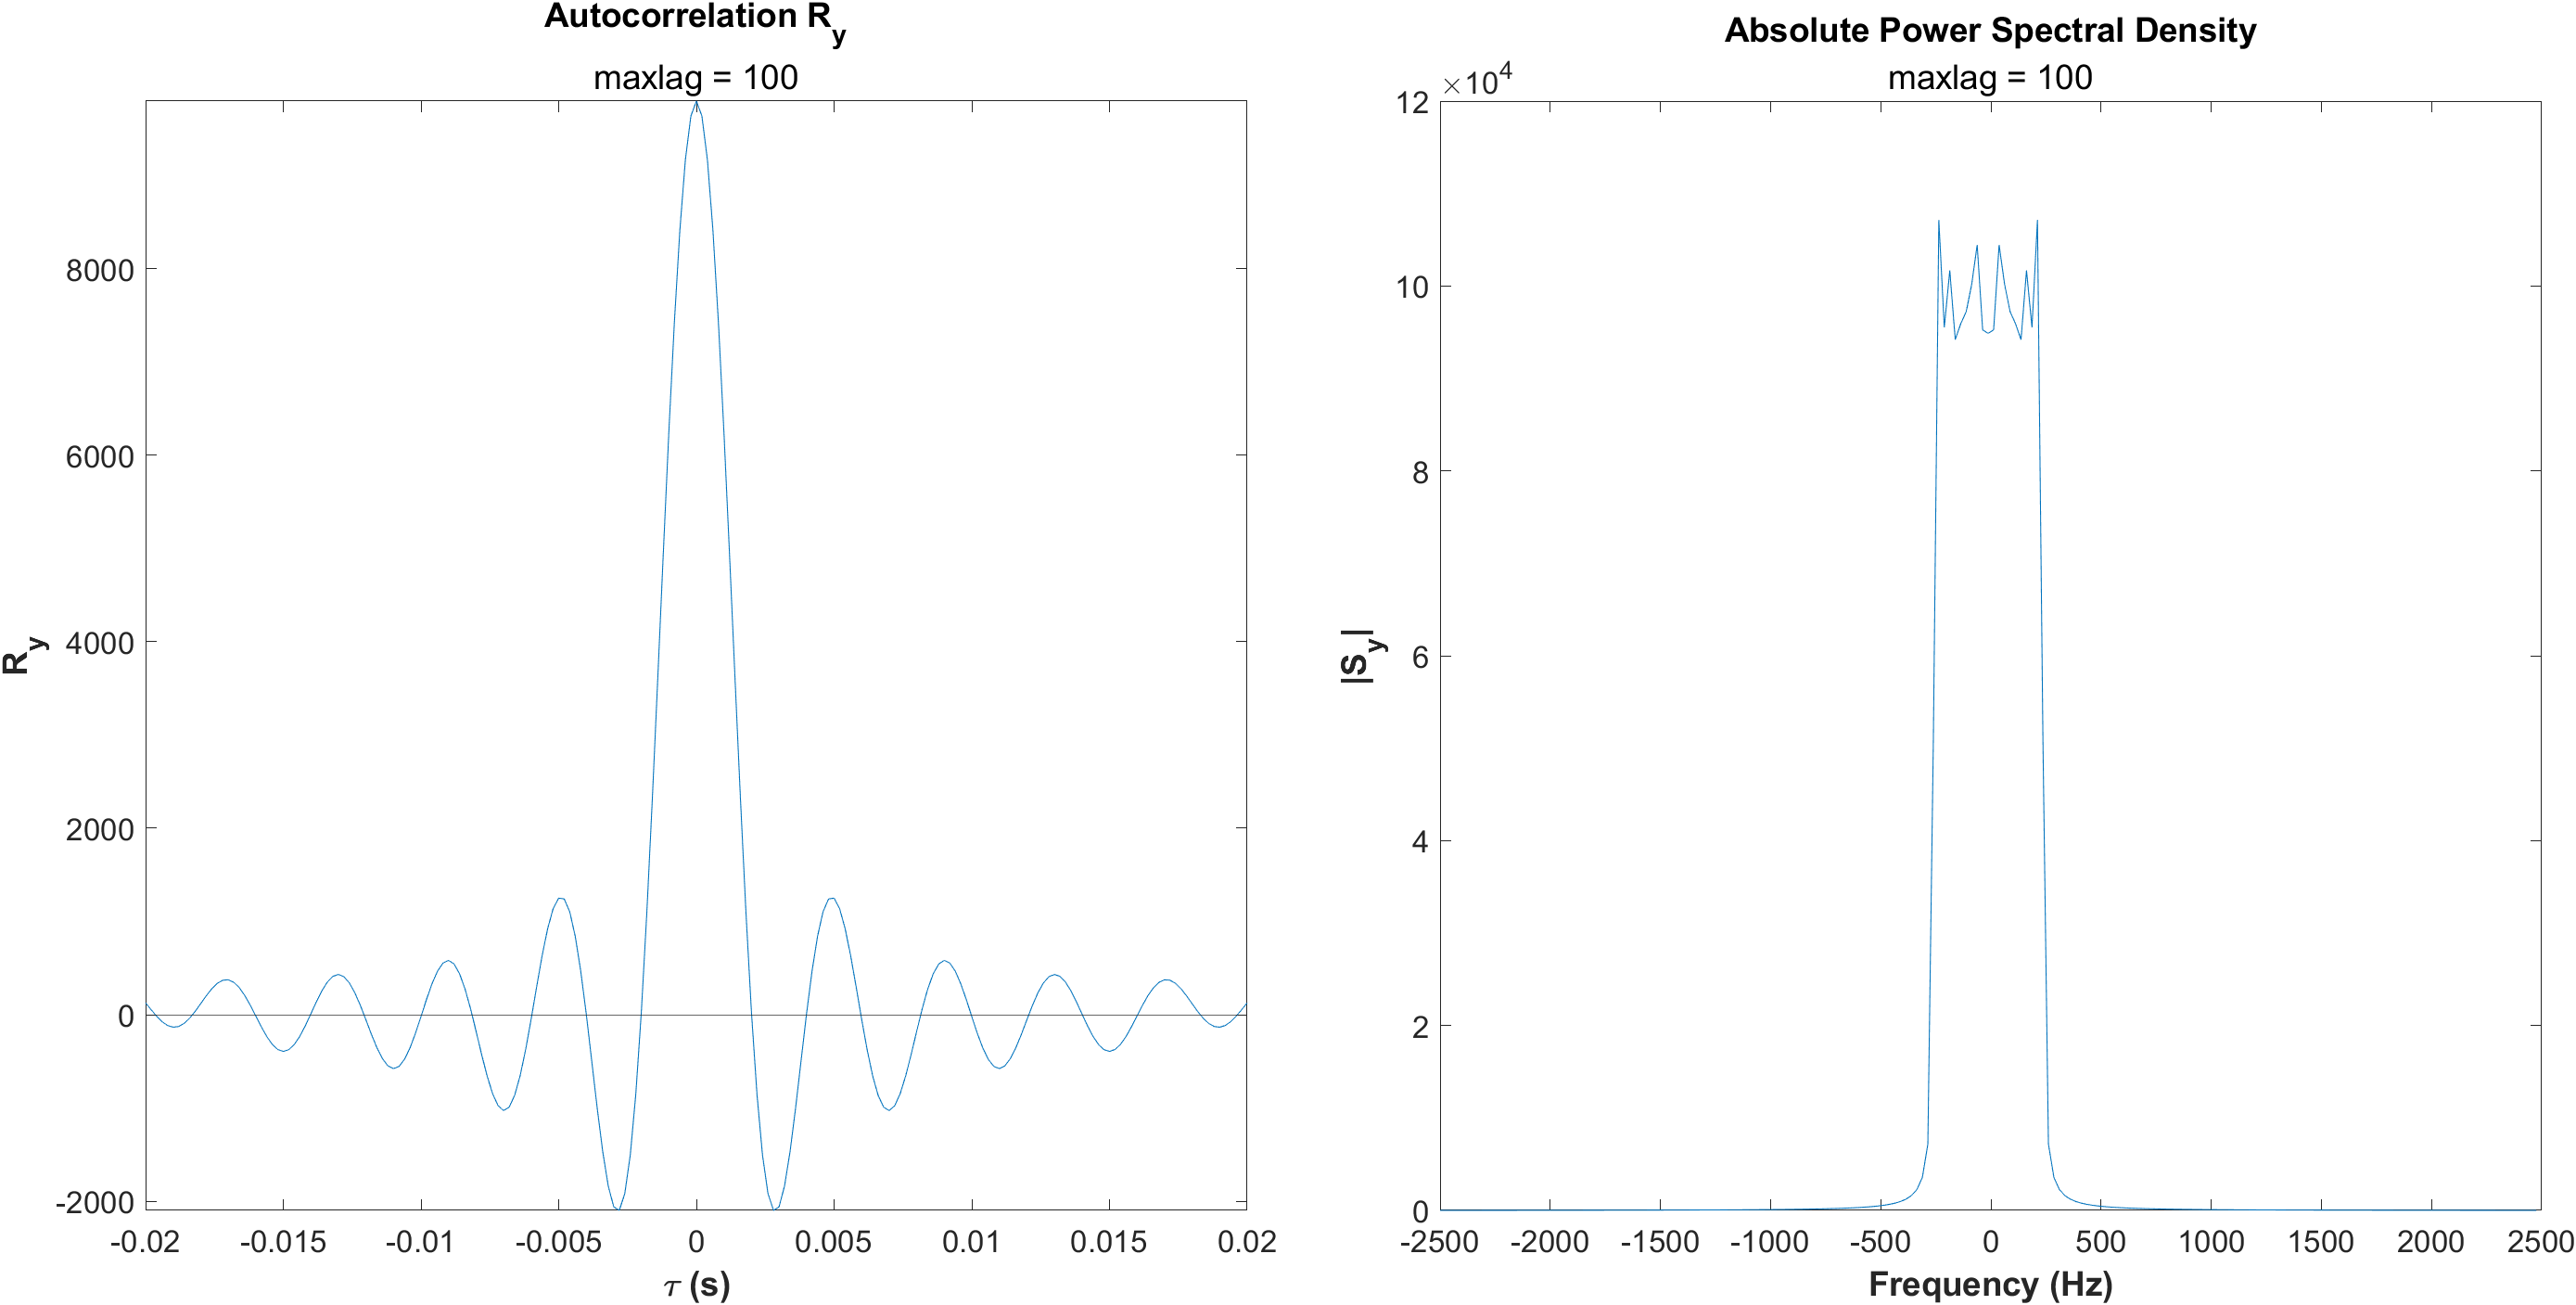
\includegraphics[width=\textwidth]{exp1_maxlag_100}
	\caption{\label{fig:exp1_maxlag100}Autocorrelation and PSD for maxlag = 100}
\end{figure}

\begin{figure}[h]
	\centering
	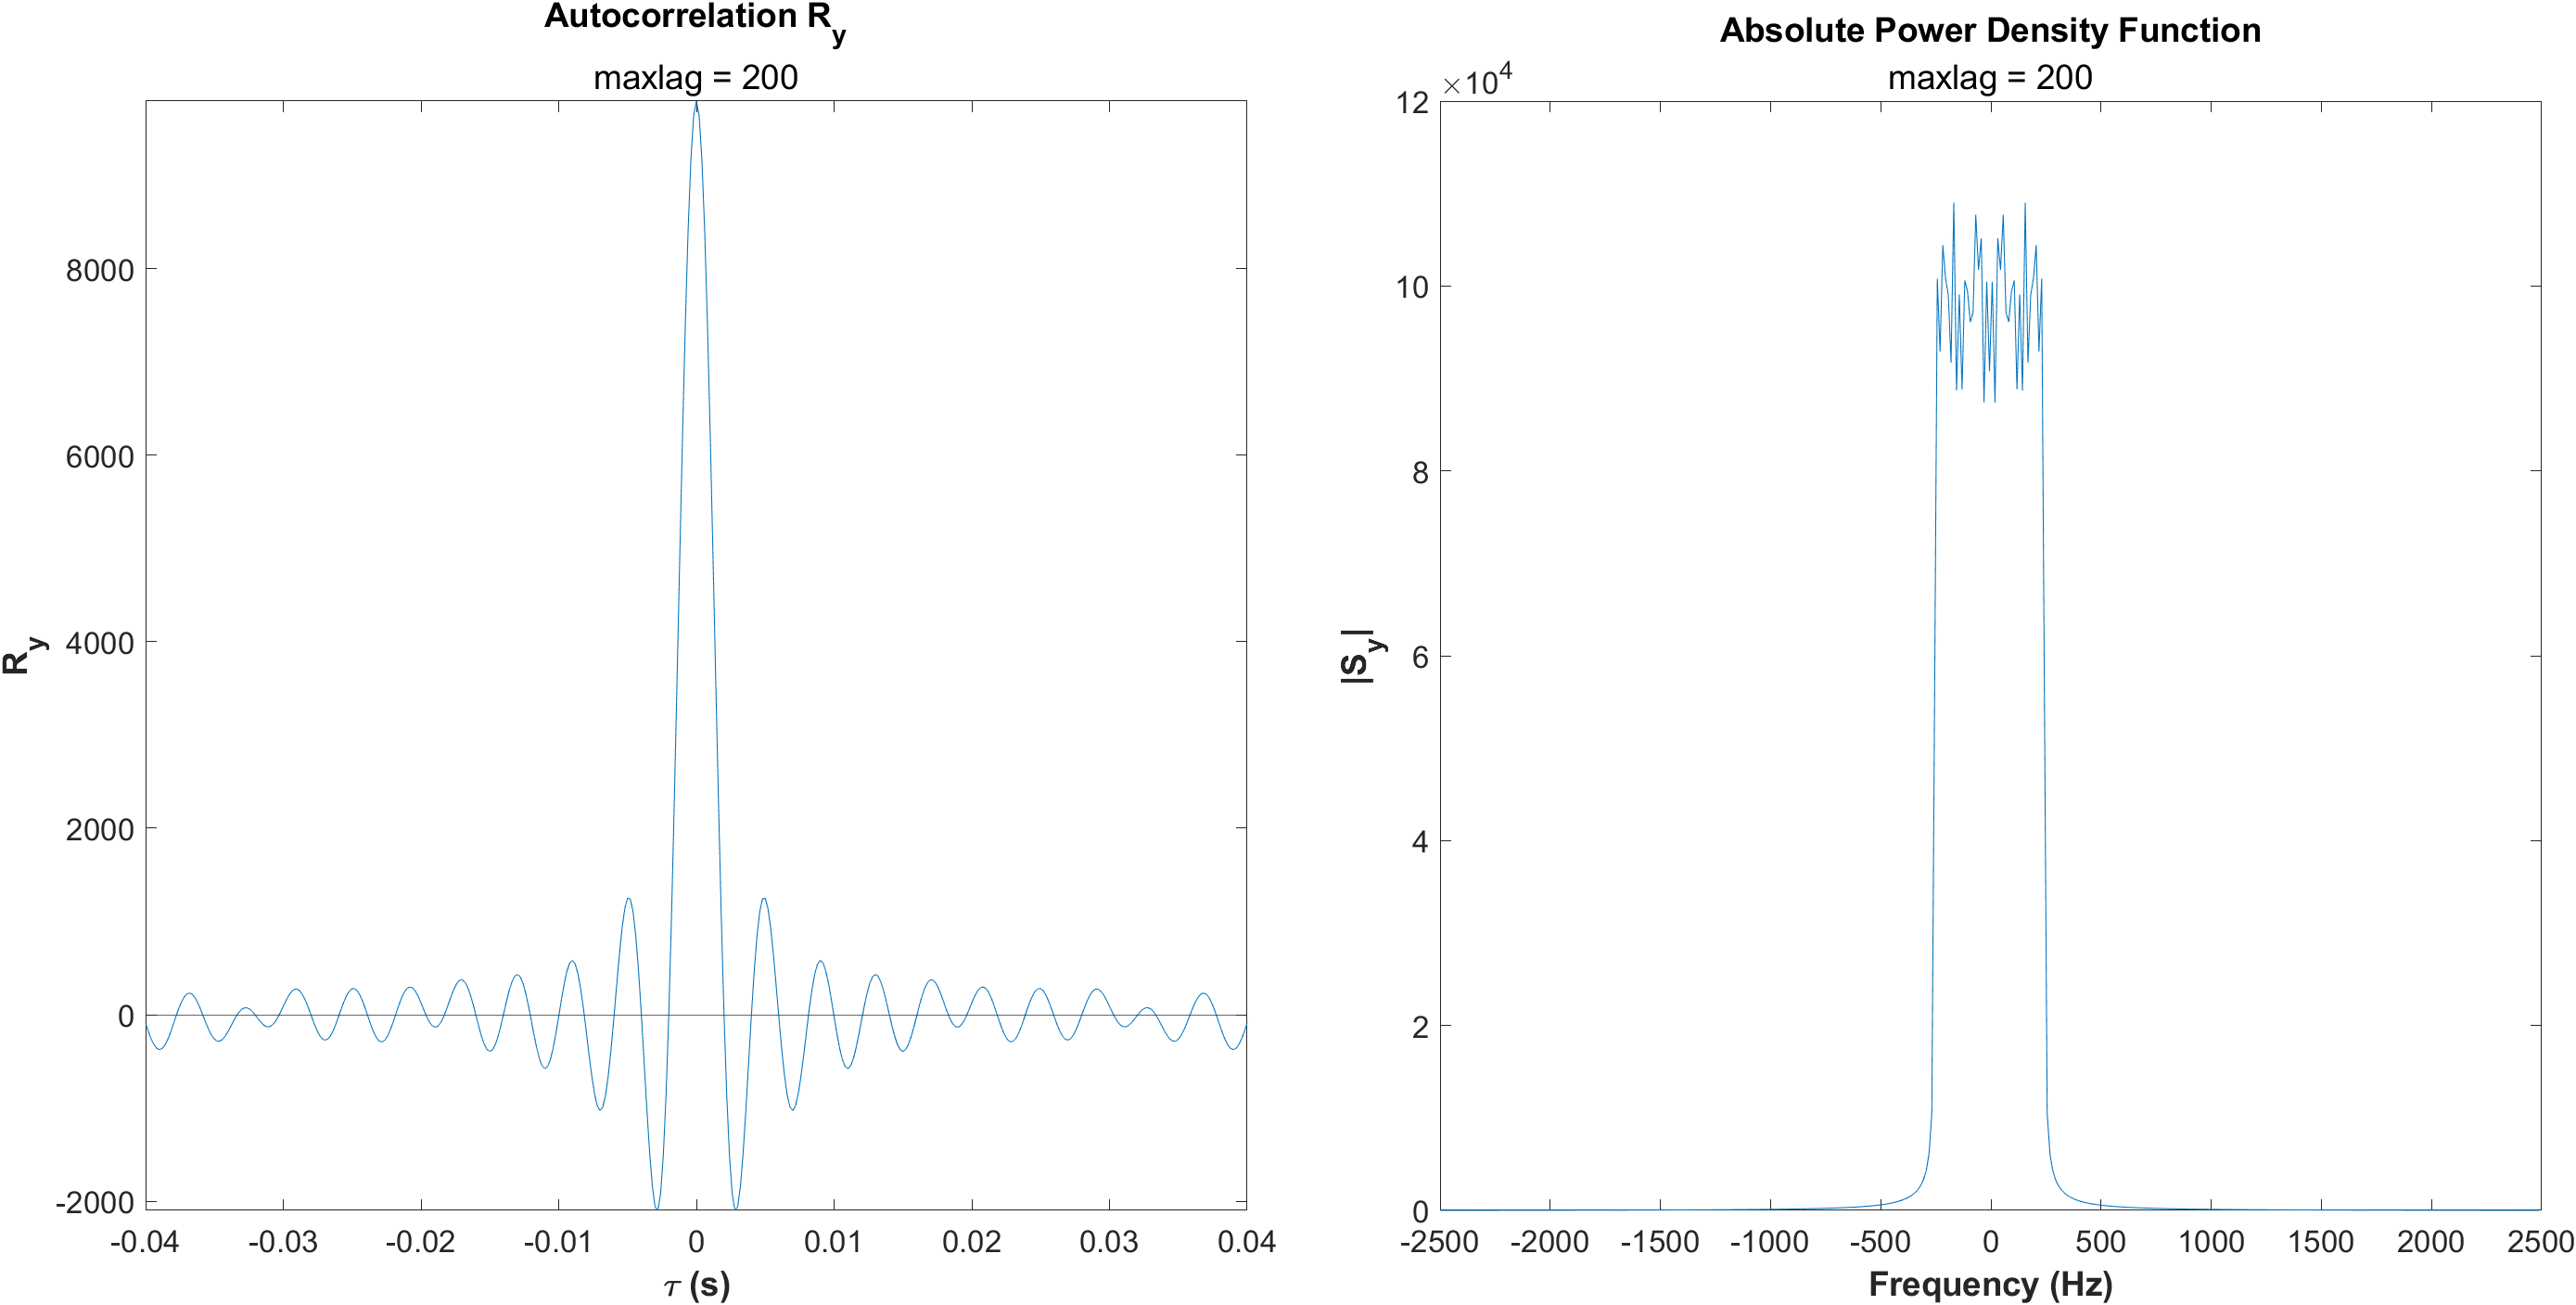
\includegraphics[width=\textwidth]{exp1_maxlag_200}
	\caption{\label{fig:exp1_maxlag200}Autocorrelation and PSD for maxlag = 200}
\end{figure}

\begin{figure}[h]
	\centering
	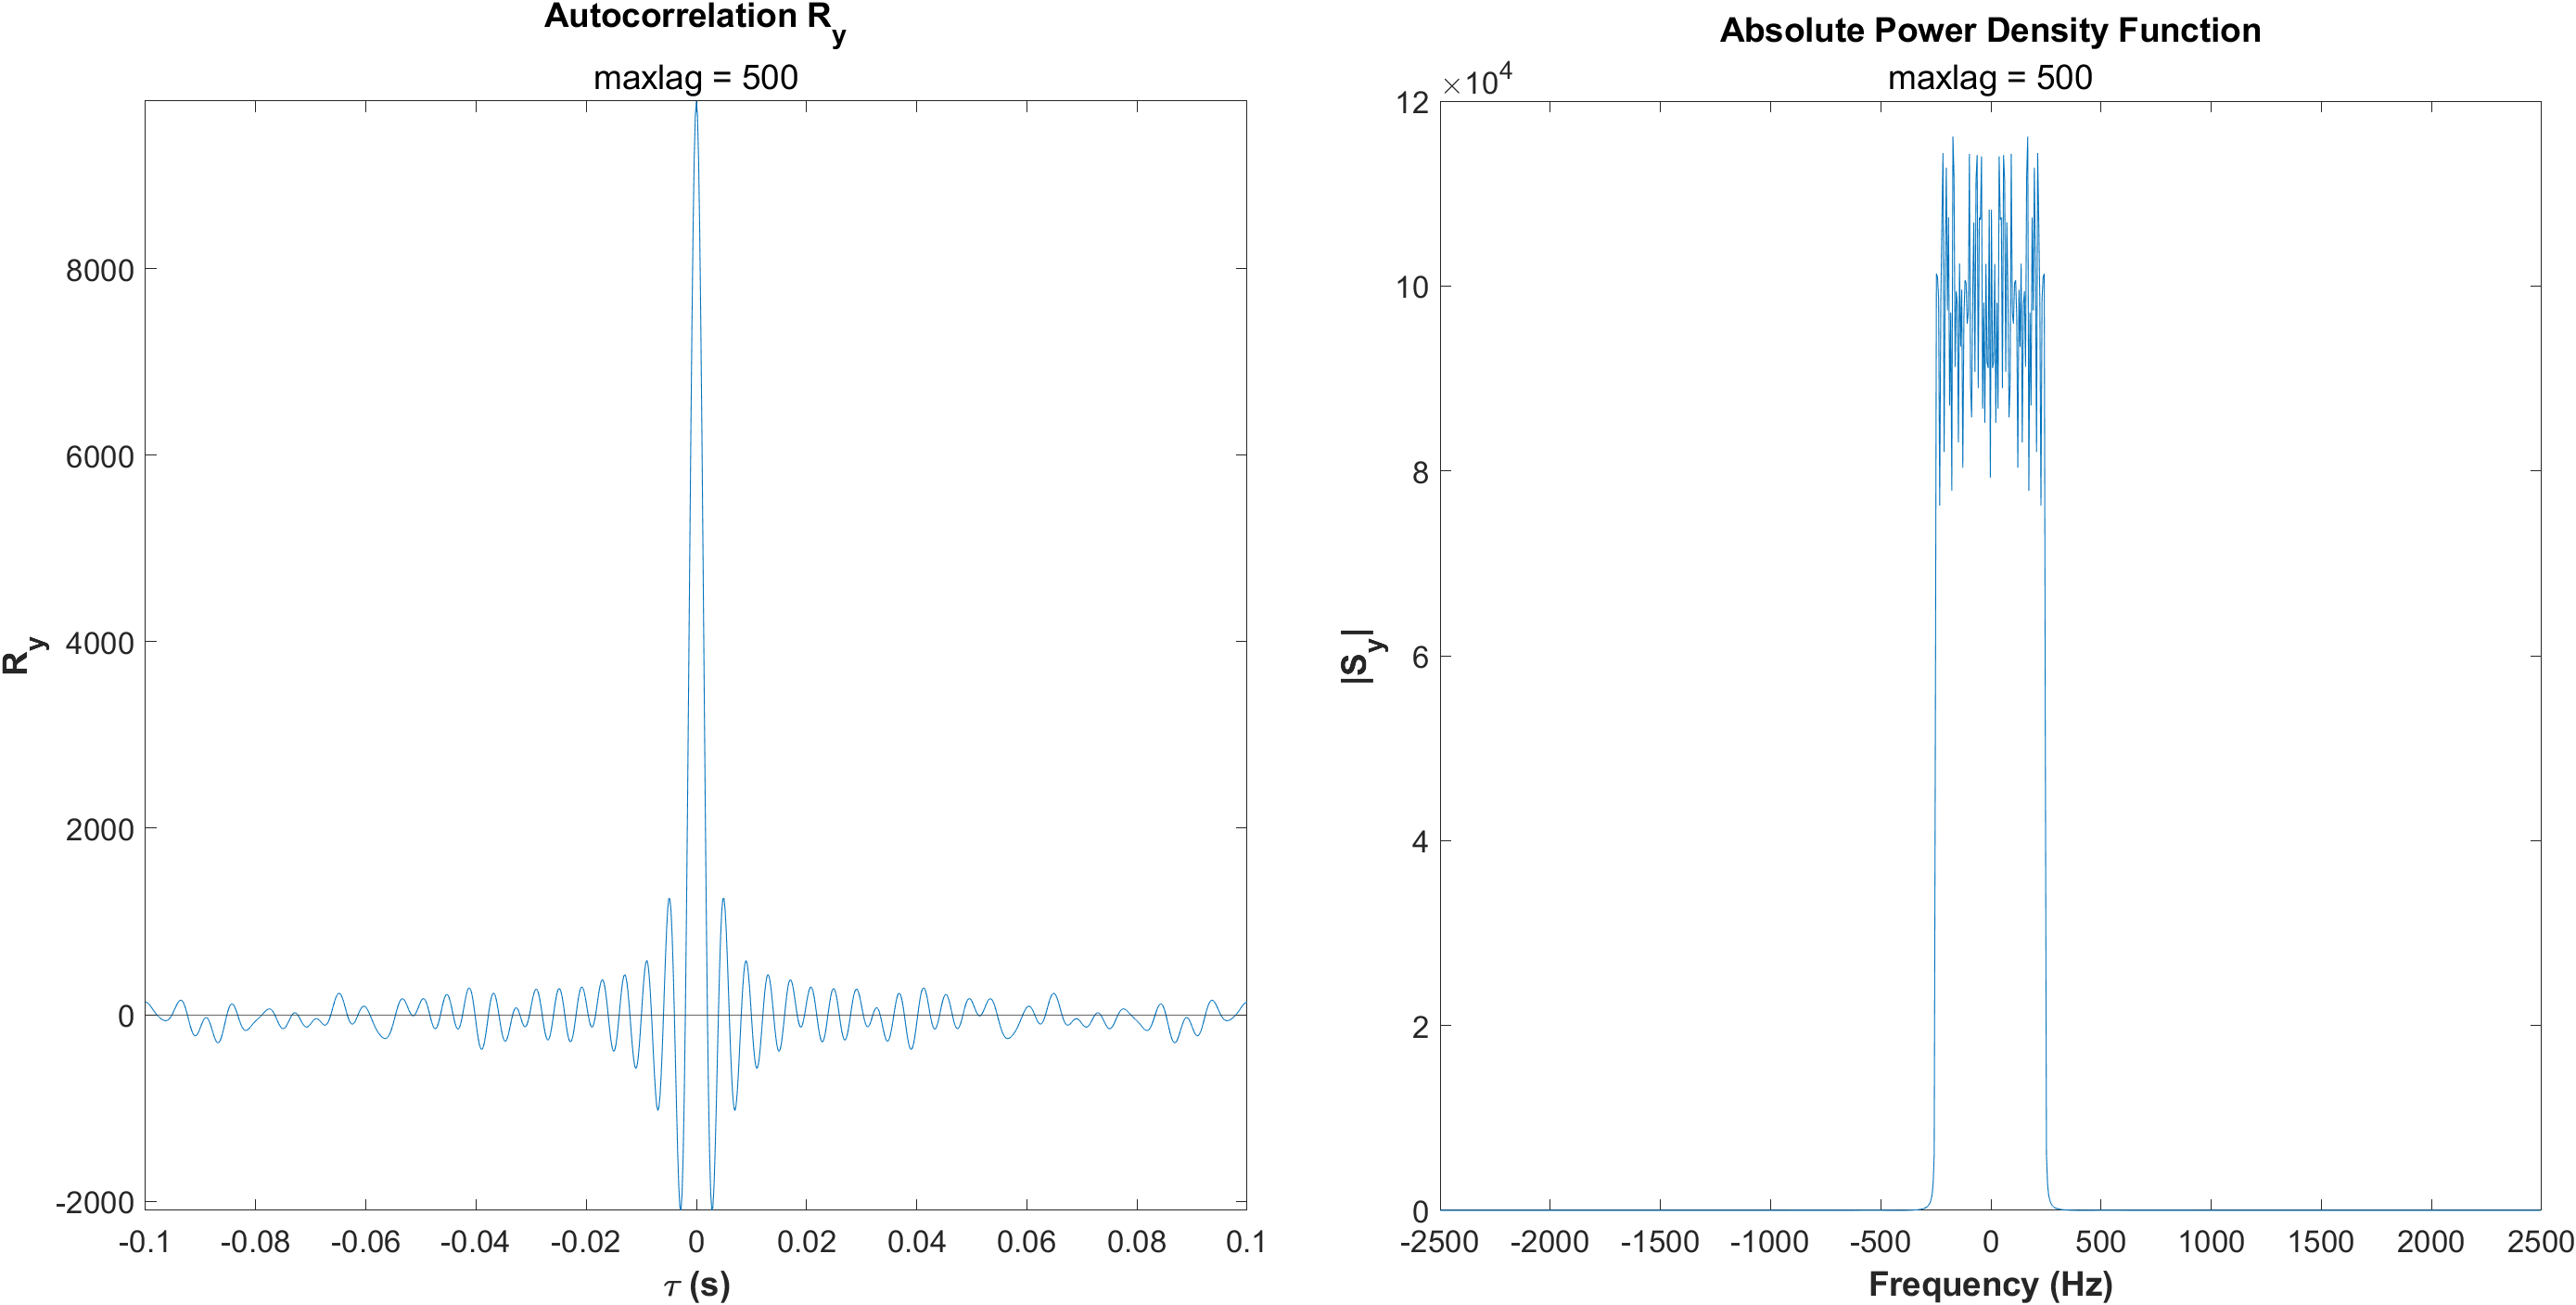
\includegraphics[width=\textwidth]{exp1_maxlag_500}
	\caption{\label{fig:exp1_maxlag500}Autocorrelation and PSD for maxlag = 500}
\end{figure}

% (iii) Estimate the bandwidth of the filter using the autocorrelation plot. Hint: measure the locations of zeros of sinc and compare it with the theoretical calculation. 

\section*{Numerical Experiment \#2: A sinusoid buried in noise}

% For this section, provide the theoretical calculations (i.e. derivations of analytical expressions for autocorrelation and PSD of the AWGN channel output. Refer to lecture notes). Compare the theoretical autocorrelation function and PSD with those from your program (qualitatively).

% (i) Do you observe a peak at the zero lag in the autocorrelation plot? Explain its origin.

% (ii) Change the maxlag from 100 to 200 and then to 20000and observe its impact on the frequency resolution. Estimating the frequency, fc in the frequency domain and provide a table of measurements for the maxlag of 100, 200 and 20000. Do the frequency estimates converge? Explain the connection between the maxlog and frequency resolution.

\begin{figure}[h]
	\centering
	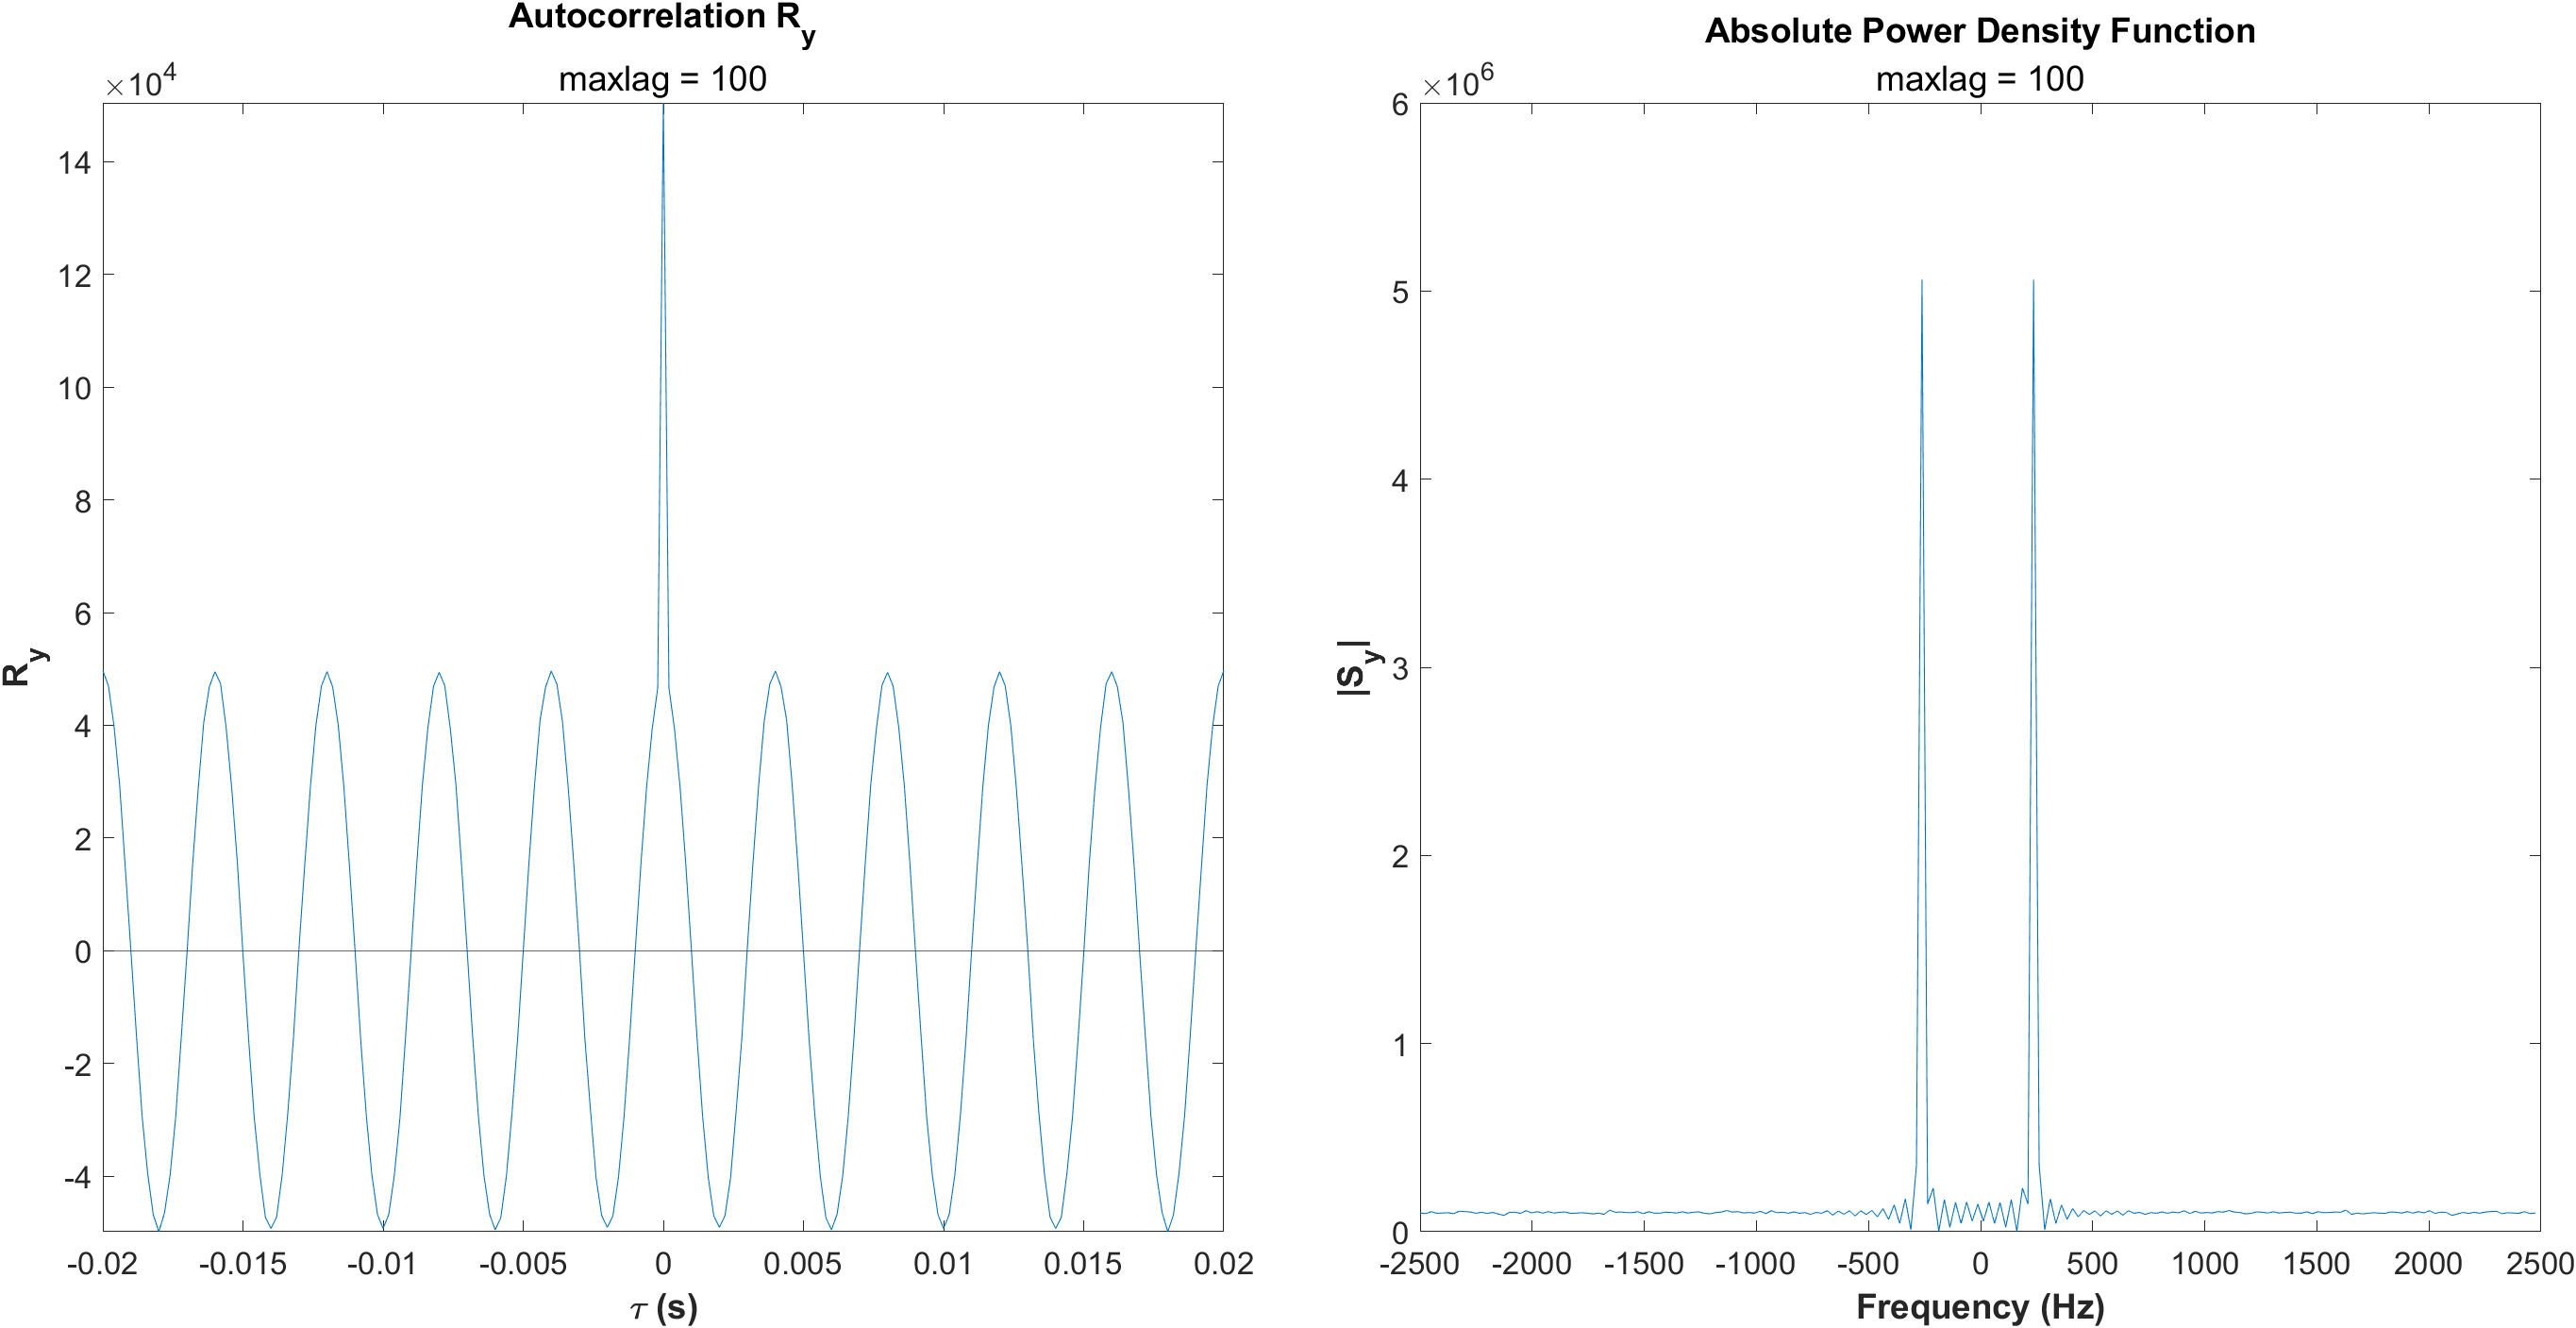
\includegraphics[width=\textwidth]{exp2_maxlag_100}
	\caption{\label{fig:exp2_maxlag100}Autocorrelation and PSD for maxlag = 100}
\end{figure}

\begin{figure}[h]
	\centering
	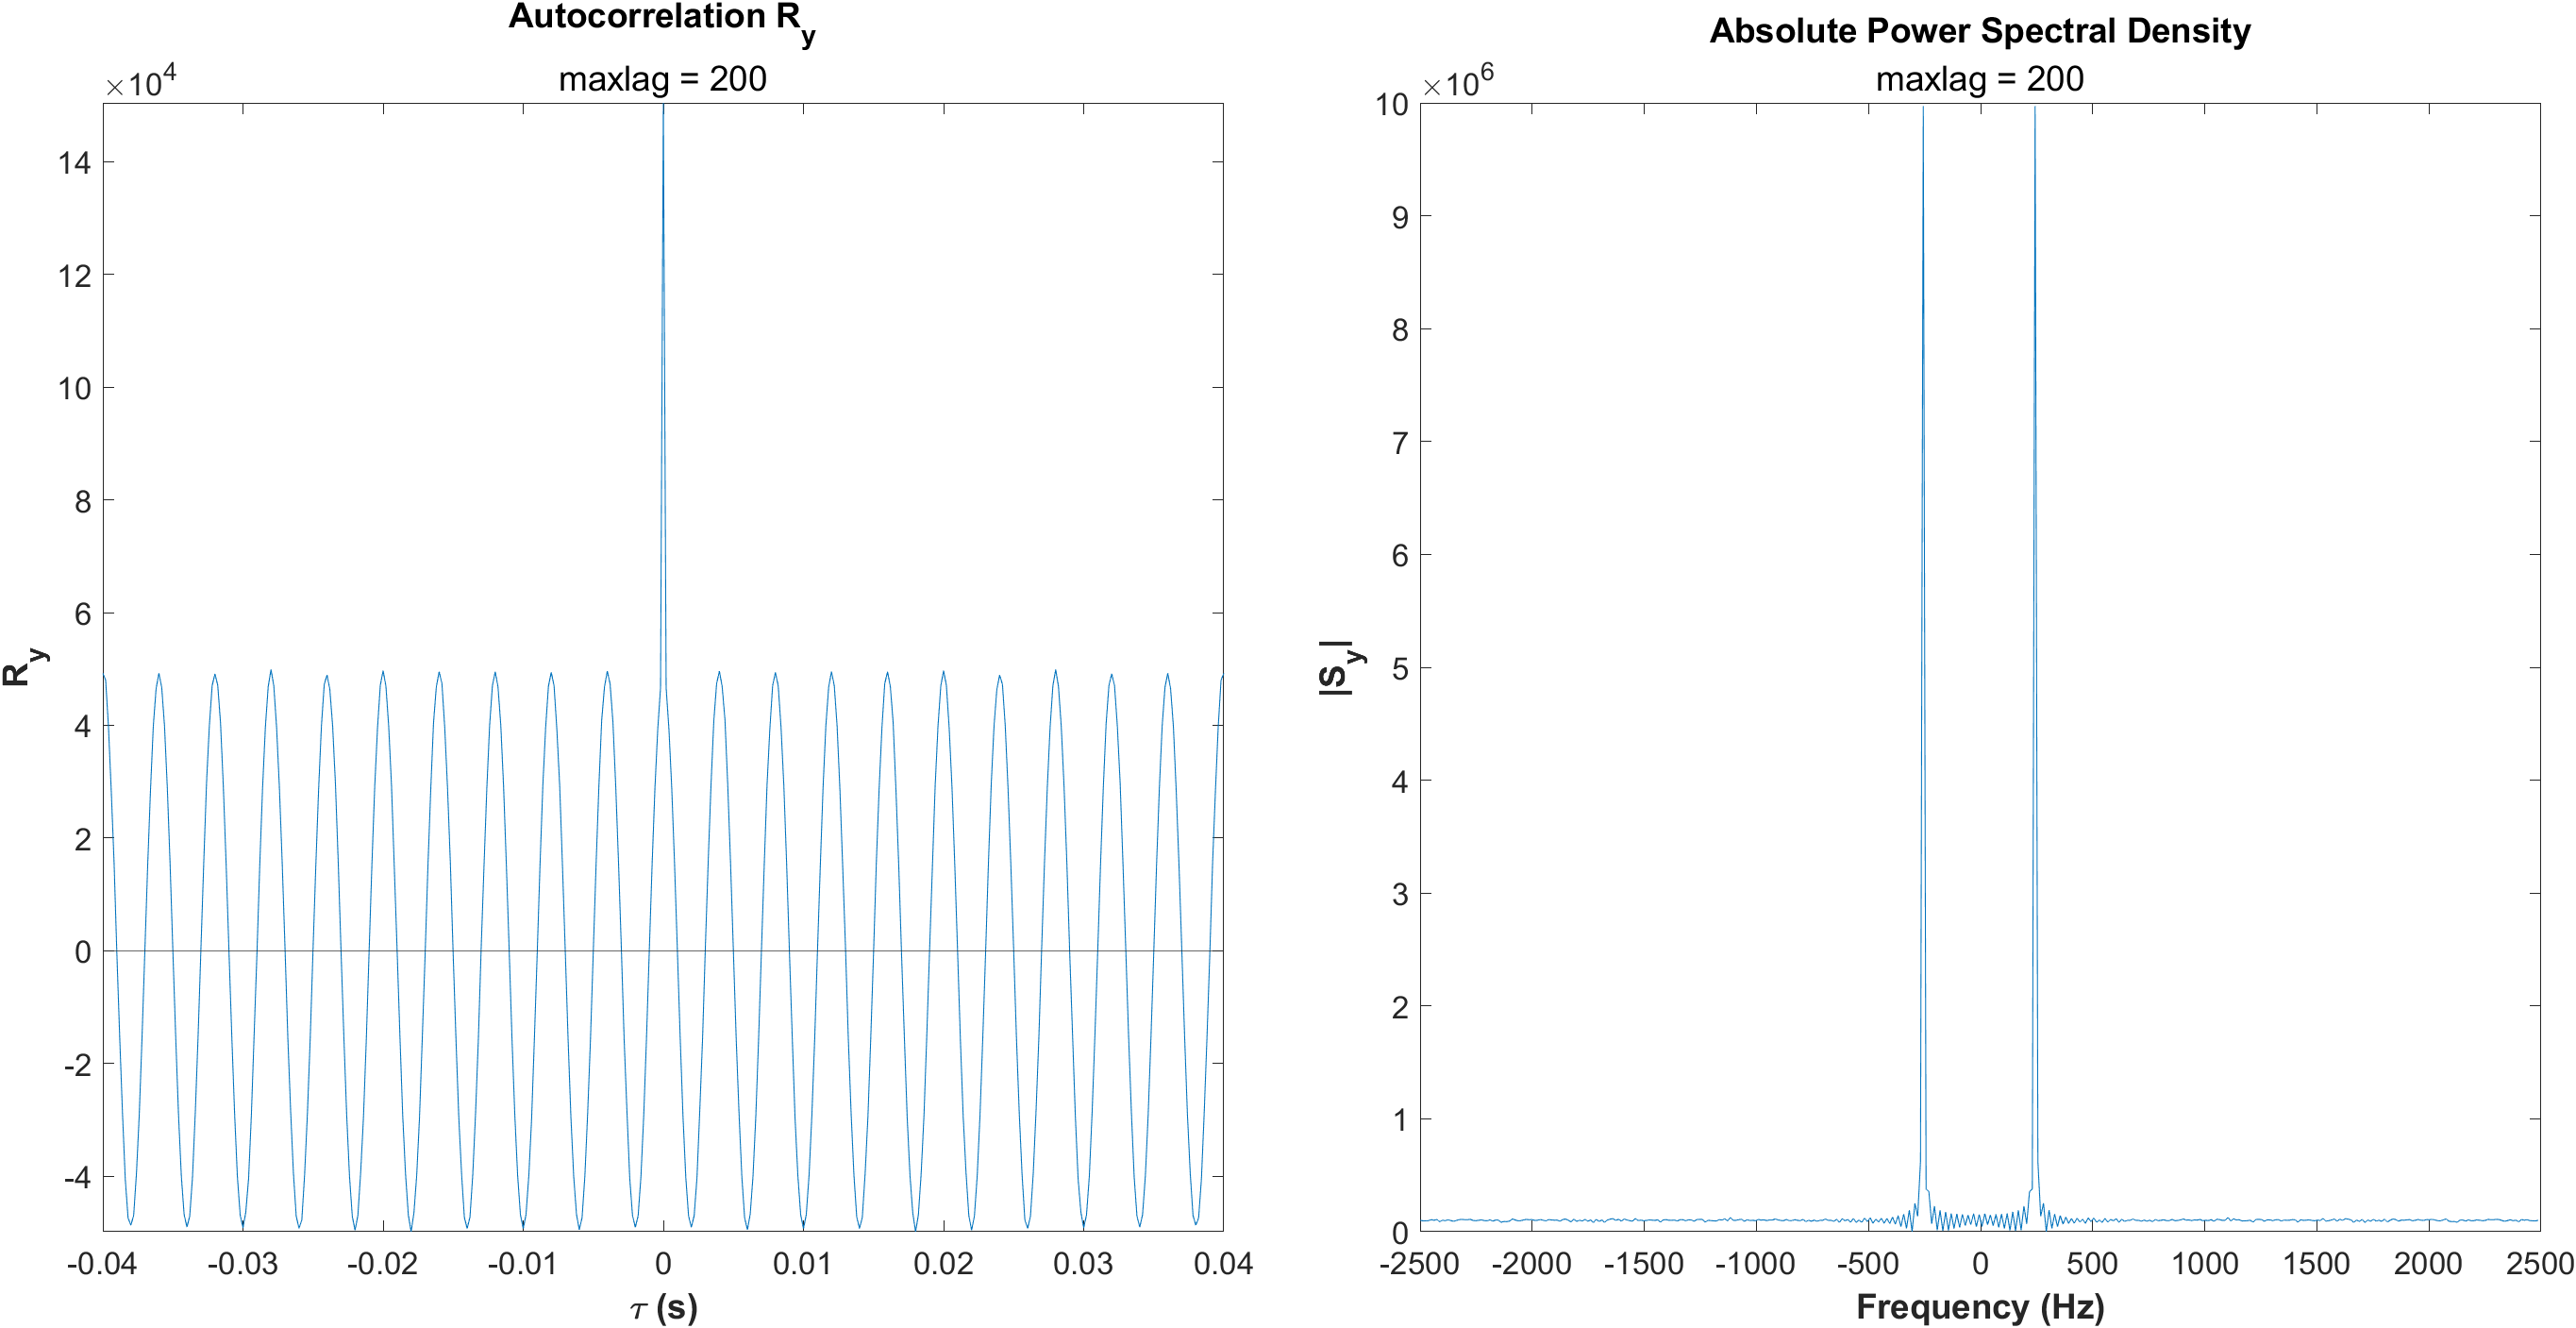
\includegraphics[width=\textwidth]{exp2_maxlag_200}
	\caption{\label{fig:exp2_maxlag200}Autocorrelation and PSD for maxlag = 200}
\end{figure}

\begin{figure}[h]
	\centering
	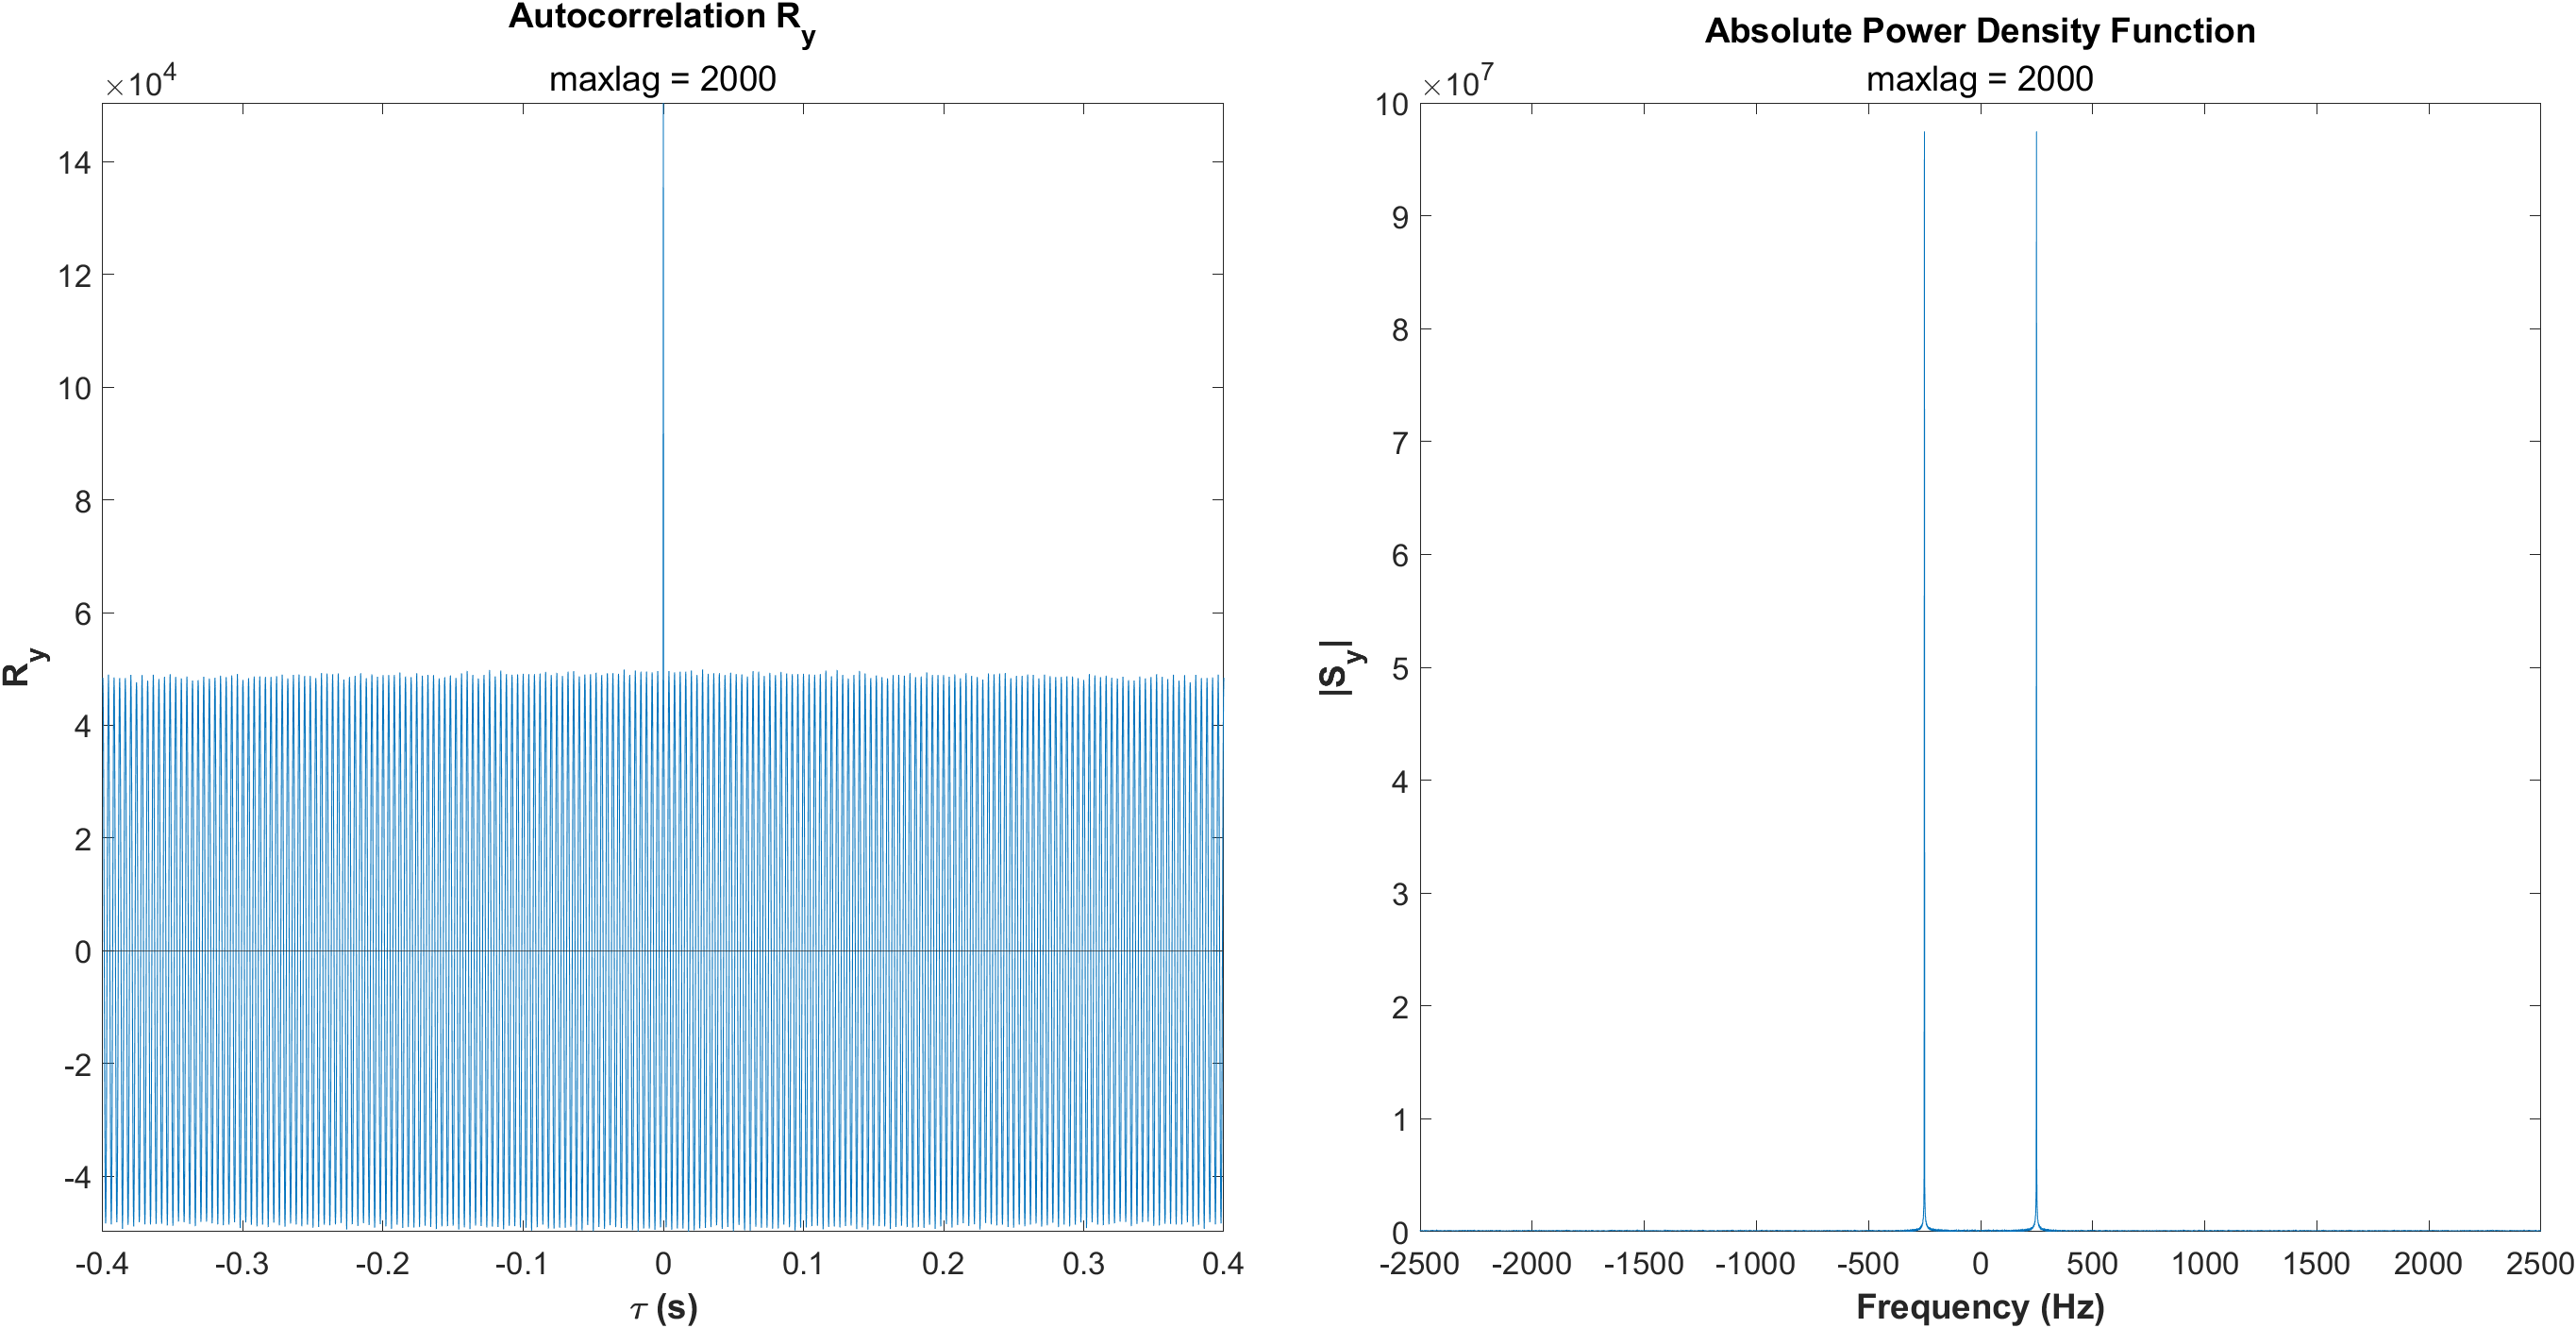
\includegraphics[width=\textwidth]{exp2_maxlag_2000}
	\caption{\label{fig:exp2_maxlag2000}Autocorrelation and PSD for maxlag = 2000}
\end{figure}

% (iii) Plot yt as a function of time. It is the sinusoidal signal buried in noise (i.e. x(t) plus white noise). Can you estimate the frequency, fc directly from yt, without calculating the correlation? Explain.

\begin{figure}[h]
	\centering
	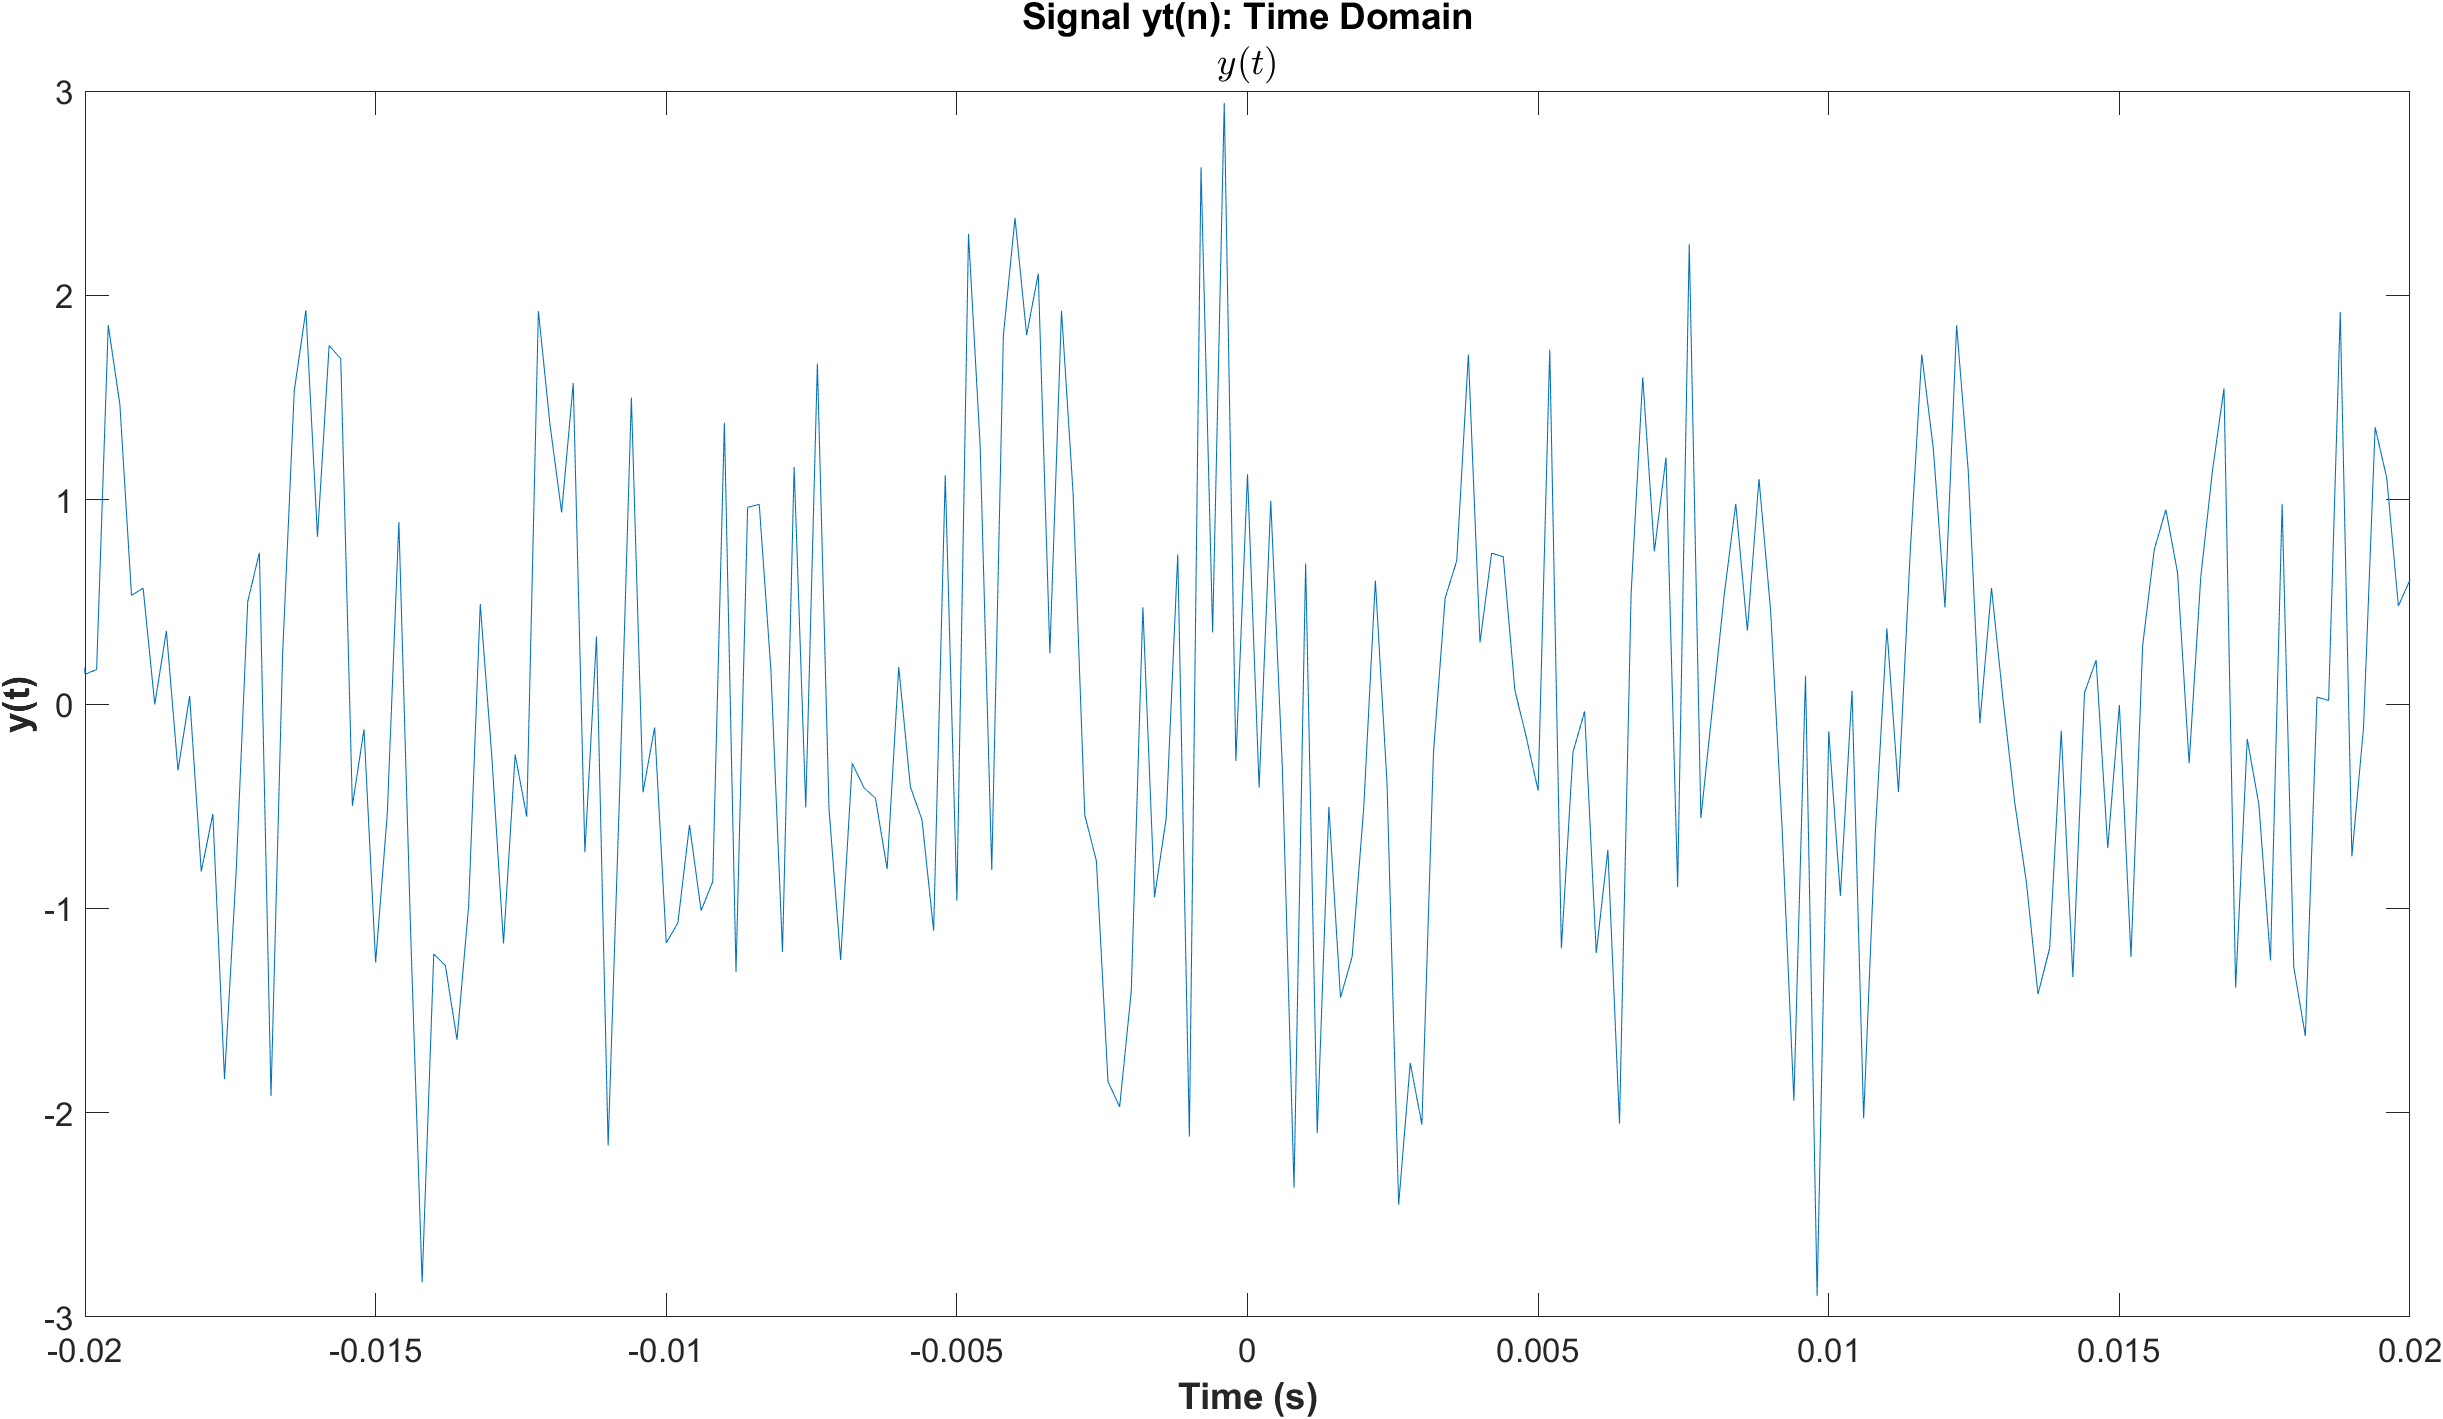
\includegraphics[width=\textwidth]{exp2_time}
	\caption{\label{fig:exp2_time}Time Domain}
\end{figure}

\section*{Numerical Experiment \#3: Delay Estimation}

% For this section, plot x(t) and y(t) vs time. Explain why your technique works and the straightforward approach of finding the delay by plotting y(t) vs time fails. Provide the plot of cross-correlation between x and y. Can you estimate the delay by the autocorrelation of y(i.e. xcorr(y,y))? Explain.

\begin{figure}[h]
	\centering
	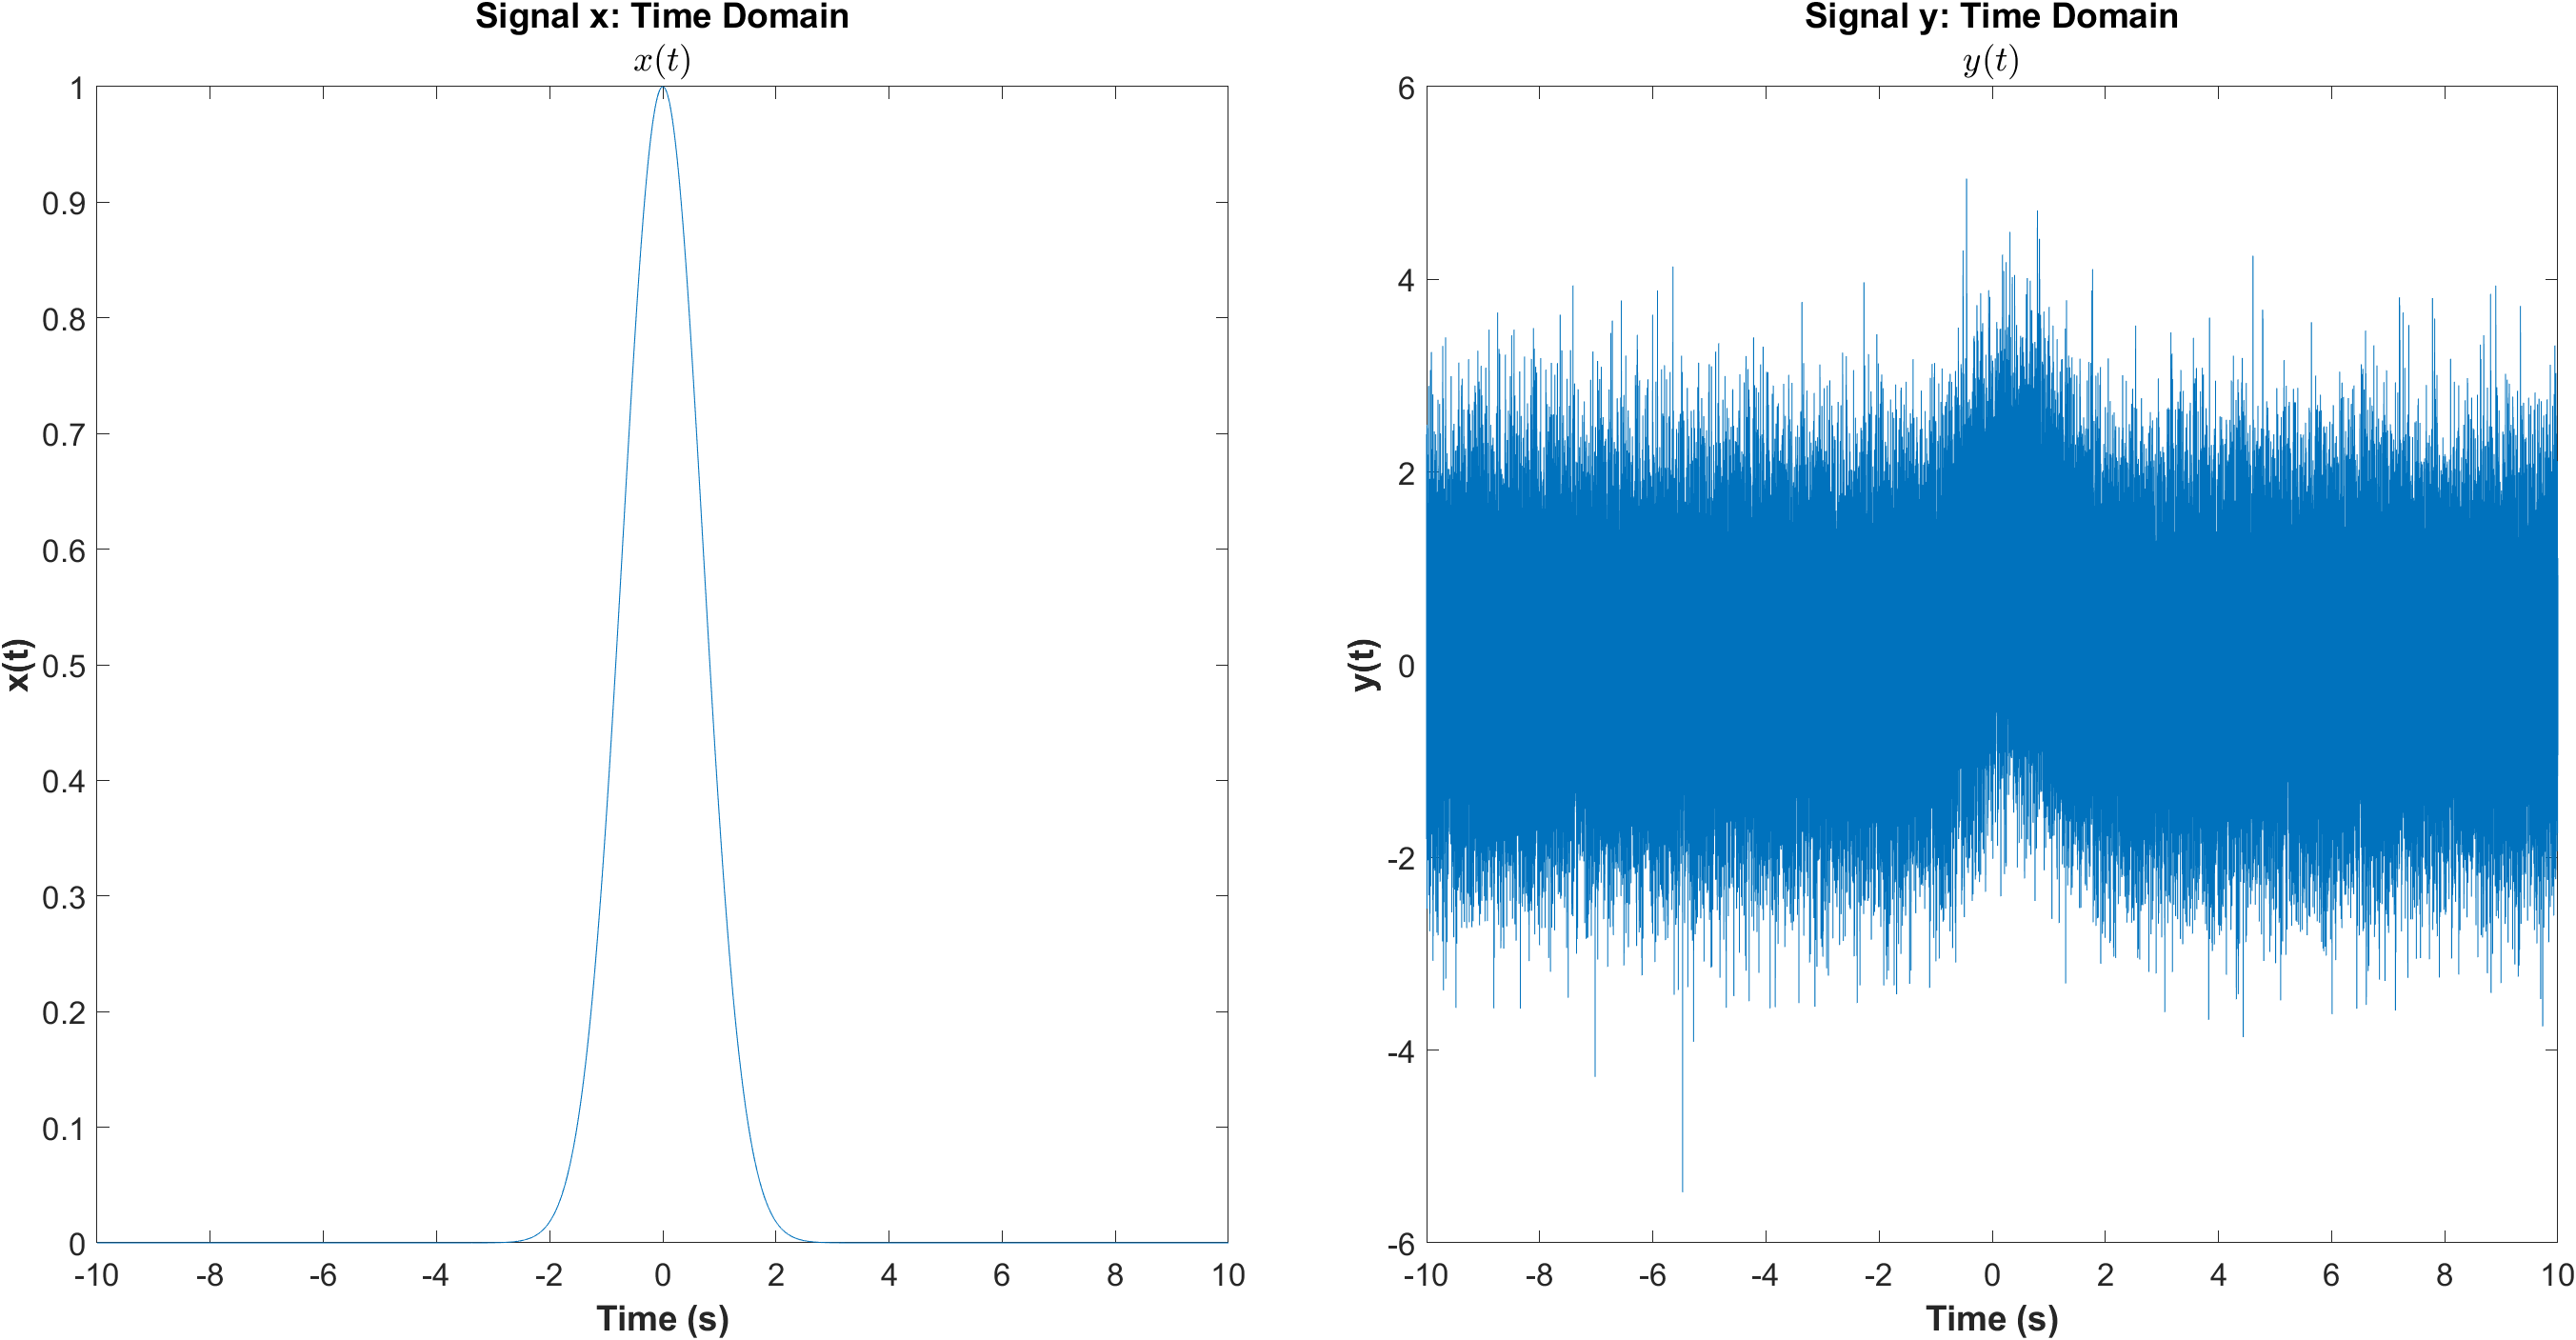
\includegraphics[width=\textwidth]{exp3_time}
	\caption{\label{fig:exp3_time}Time Domain}
\end{figure}

\begin{figure}[h]
	\centering
	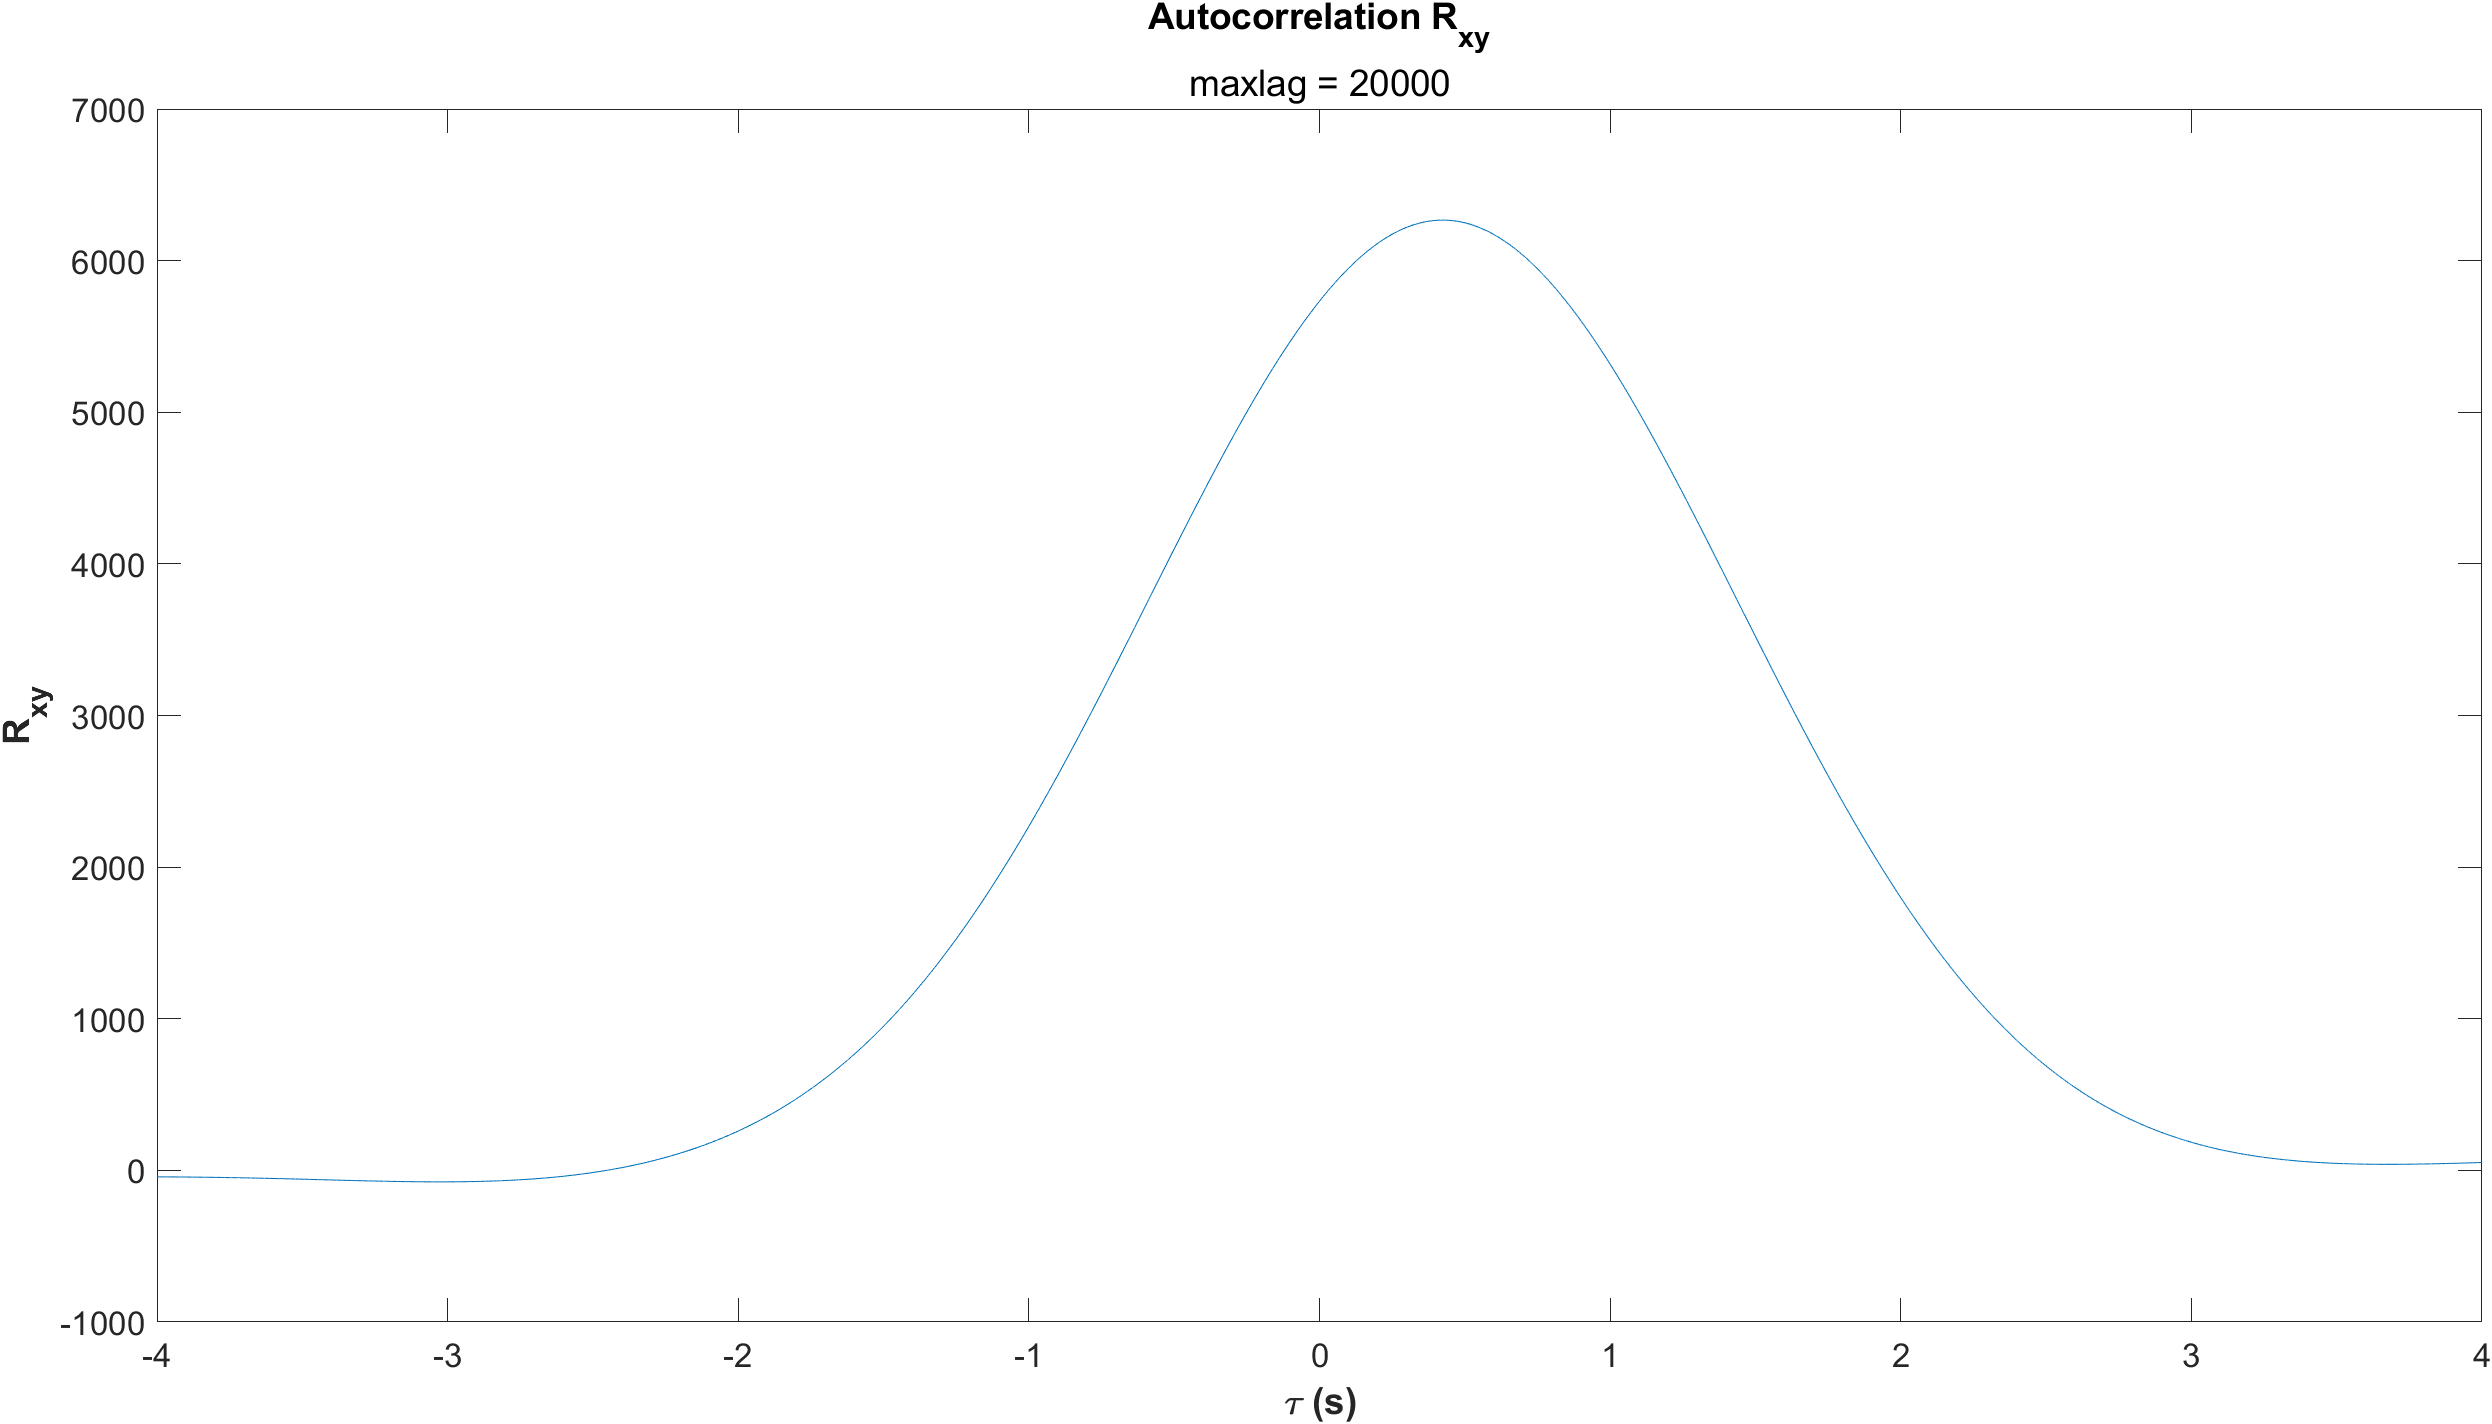
\includegraphics[width=\textwidth]{exp3_autocorr}
	\caption{\label{fig:exp3_autocorr}Autocorrelation}
\end{figure}

\end{document}